% !TEX TS-program = XeLaTeX
% use the following command:
% all document files must be coded in UTF-8
\documentclass[english]{textolivre}
% build HTML with: make4ht -e build.lua -c textolivre.cfg -x -u article "fn-in,svg,pic-align"

\journalname{Texto Livre}
\thevolume{17}
%\thenumber{1} % old template
\theyear{2024}
\receiveddate{\DTMdisplaydate{2023}{5}{15}{-1}} % YYYY MM DD
\accepteddate{\DTMdisplaydate{2023}{6}{28}{-1}}
\publisheddate{\DTMdisplaydate{2023}{10}{31}{-1}}
\corrauthor{Rafael Zaccaron}
\articledoi{10.1590/1983-3652.2024.46202}
%\articleid{NNNN} % if the article ID is not the last 5 numbers of its DOI, provide it using \articleid{} commmand 
% list of available sesscions in the journal: articles, dossier, reports, essays, reviews, interviews, editorial
\articlesessionname{dossier}
\runningauthor{Xhafaj and Zaccaron} 
%\editorname{Leonardo Araújo} % old template
\sectioneditorname{Daniervelin Pereira}
\layouteditorname{Thaís Coutinho}

\title{Online peer conferences: a window of opportunities for feedback on writing}
\othertitle{Conferência \textit{online} entre pares: uma janela de oportunidade a favor do \textit{feedback} para a escrita}
% if there is a third language title, add here:
%\othertitle{Artikelvorlage zur Einreichung beim Texto Livre Journal}

\author[1]{Donesca Cristina Puntel Xhafaj~\orcid{0000-0002-2560-2919}\thanks{Email: \href{mailto:donesca@hotmail.com}{donesca@hotmail.com}}}
\author[1]{Rafael Zaccaron~\orcid{0000-0001-7796-501X}\thanks{Email: \href{mailto:rafaelzaccaron@gmail.com}{rafaelzaccaron@gmail.com}}}
\affil[1]{Universidade Federal de Santa Catarina, Centro de Comunicação e Expressão, Florianópolis, SC, Brasil.}

\addbibresource{article.bib}
% use biber instead of bibtex
% $ biber article

% used to create dummy text for the template file
\definecolor{dark-gray}{gray}{0.35} % color used to display dummy texts
\usepackage{lipsum}
\SetLipsumParListSurrounders{\colorlet{oldcolor}{.}\color{dark-gray}}{\color{oldcolor}}

% used here only to provide the XeLaTeX and BibTeX logos
\usepackage{hologo}

% if you use multirows in a table, include the multirow package
\usepackage{multirow}

% provides sidewaysfigure environment
\usepackage{rotating}

% CUSTOM EPIGRAPH - BEGIN 
%%% https://tex.stackexchange.com/questions/193178/specific-epigraph-style
\usepackage{epigraph}
\renewcommand\textflush{flushright}
\makeatletter
\newlength\epitextskip
\pretocmd{\@epitext}{\em}{}{}
\apptocmd{\@epitext}{\em}{}{}
\patchcmd{\epigraph}{\@epitext{#1}\\}{\@epitext{#1}\\[\epitextskip]}{}{}
\makeatother
\setlength\epigraphrule{0pt}
\setlength\epitextskip{0.5ex}
\setlength\epigraphwidth{.7\textwidth}
% CUSTOM EPIGRAPH - END

% LANGUAGE - BEGIN
% ARABIC
% for languages that use special fonts, you must provide the typeface that will be used
% \setotherlanguage{arabic}
% \newfontfamily\arabicfont[Script=Arabic]{Amiri}
% \newfontfamily\arabicfontsf[Script=Arabic]{Amiri}
% \newfontfamily\arabicfonttt[Script=Arabic]{Amiri}
%
% in the article, to add arabic text use: \textlang{arabic}{ ... }
%
% RUSSIAN
% for russian text we also need to define fonts with support for Cyrillic script
% \usepackage{fontspec}
% \setotherlanguage{russian}
% \newfontfamily\cyrillicfont{Times New Roman}
% \newfontfamily\cyrillicfontsf{Times New Roman}[Script=Cyrillic]
% \newfontfamily\cyrillicfonttt{Times New Roman}[Script=Cyrillic]
%
% in the text use \begin{russian} ... \end{russian}
% LANGUAGE - END

% EMOJIS - BEGIN
% to use emoticons in your manuscript
% https://stackoverflow.com/questions/190145/how-to-insert-emoticons-in-latex/57076064
% using font Symbola, which has full support
% the font may be downloaded at:
% https://dn-works.com/ufas/
% add to preamble:
% \newfontfamily\Symbola{Symbola}
% in the text use:
% {\Symbola }
% EMOJIS - END

% LABEL REFERENCE TO DESCRIPTIVE LIST - BEGIN
% reference itens in a descriptive list using their labels instead of numbers
% insert the code below in the preambule:
%\makeatletter
%\let\orgdescriptionlabel\descriptionlabel
%\renewcommand*{\descriptionlabel}[1]{%
%  \let\orglabel\label
%  \let\label\@gobble
%  \phantomsection
%  \edef\@currentlabel{#1\unskip}%
%  \let\label\orglabel
%  \orgdescriptionlabel{#1}%
%}
%\makeatother
%
% in your document, use as illustraded here:
%\begin{description}
%  \item[first\label{itm1}] this is only an example;
%  % ...  add more items
%\end{description}
% LABEL REFERENCE TO DESCRIPTIVE LIST - END


% add line numbers for submission
%\usepackage{lineno}
%\linenumbers

\begin{document}
\maketitle

\begin{polyabstract}
\begin{abstract}
The pandemic has had quite an impact on the way we teach and learn. During that time, Brazilian universities implemented remote learning for more than 15 months. While the initial move was a reaction to an emergency and saw the transposition of many classes to the virtual mode, the following months saw the flourishing of initiatives that enhanced learning by streamlining the use of digital technology. In this context, this descriptive qualitative study employs an exploratory multiple case approach to investigate the affordances in the digital context tertiary students use to facilitate engagement with computer-mediated peer feedback during a course of academic literacies in English at a university in Brazil. Data come from individual semi-structured interviews, online peer-to-peer feedback meeting recordings, and retrospective individual interviews with three pairs of students. The participants are tertiary learners who had two online meetings, using Google Meet, to discuss their peer feedback on two texts they wrote for the course over one semester. Results indicate that online peer conferences offer a multimodal communication channel where different semiotic aspects play a role in mediating written input. In addition, WhatsApp was extensively used for informal peer feedback. We conclude with pedagogical implications and suggest actions so that learners can harness the full potential offered by these tools.

\keywords{Peer feedback \sep Online peer conference \sep Academic writing \sep Academic literacies \sep Google Meet}
\end{abstract}

\begin{portuguese}
\begin{abstract}
 A pandemia teve um grande impacto na forma como ensinamos e aprendemos. Durante esse tempo, as universidades brasileiras implementaram o ensino remoto por mais de 15 meses. Se inicialmente esse movimento foi uma reação emergencial e observou-se a transposição de muitas aulas presenciais para o modo virtual, nos meses seguintes observaram-se novas iniciativas que potencializaram o aprendizado mobilizando de forma eficiente o uso da tecnologia digital. Nesse contexto, este estudo descritivo qualitativo emprega uma abordagem exploratória de casos múltiplos para investigar os propiciamentos no contexto digital que os alunos do ensino superior usam para facilitar o engajamento com \textit{feedback} por pares mediado por computador durante um curso de letramento acadêmico em inglês em uma universidade no Brasil. Os dados provêm de entrevistas individuais semiestruturadas, gravações de reuniões do \textit{feedback} em duplas e seções de visionamentos individuais com três pares de alunos. Os participantes são alunos do ensino superior que tiveram duas reuniões \textit{online}, usando o Google Meet, para discutir o \textit{feedback} de seus colegas sobre dois textos que escreveram para o curso ao longo de um semestre. Os resultados indicam que as conferências \textit{online} oferecem um canal de comunicação multimodal, em que diferentes aspectos semióticos desempenham um papel na mediação do insumo escrito. Além disso, o WhatsApp foi amplamente utilizado para \textit{feedback} informal de colegas. Concluímos o trabalho com implicações pedagógicas e sugerimos ações para que os aprendizes possam aproveitar todo o potencial oferecido por essas ferramentas.

\keywords{\textit{Feedback} por pares \sep Conferência \textit{online} entre pares \sep Escrita acadêmica \sep Letramento acadêmico \sep Google Meet}
\end{abstract}
\end{portuguese}
% if there is another abstract, insert it here using the same scheme
\end{polyabstract}

\section{Introduction}

Feedback, in its various forms, is not only part and parcel of the educational process but is also a multifaceted phenomenon that is most critical to learning \cite{hattie2007power}. In higher education, feedback is a valuable assessment tool that can mediate the development of academic literacies. Definitions of feedback are varied, with different focuses; we adopt \textcite[p. 1315]{carless2018development} view that feedback is “a process through which learners make sense of information from various sources and use it to enhance their work or learning strategies”. This view of feedback expands the traditional notion of a teacher being central to the feedback process, with the learner having a passive role. Moreover, by focusing on the process, we can look at how technology-enhanced tools may be a part of contemporary pedagogy related to feedback.

With the surge of the COVID-19 pandemic, many teachers who had never had any experiences with online learning were forced to switch to this modality. While synchronous meeting tools, such as Zoom, which allow for much more than lecture-type online classes \cite{kohnke2022facilitating}, were available in many contexts, especially in higher education, a great number of inexperienced professors, and perhaps even others who had already used these tools in the past, were caught unaware of the possibilities these platforms offer and ended up trying to carry out, during this period, classes that used the same procedures as the ones they employed in face-to-face contexts. Though understandable, this approach not only increased the amount of work and stress for teachers trying to adapt to the unplanned switch to remote teaching \cite{silus2020desafios} but also did not motivate learners. One of the issues was that students did not enjoy classes that were mostly PowerPoint-led and with interaction mainly between the teacher and students \cite{belda2021enhancing}. One of the most common complaints was the lack of peer-to-peer interaction in online synchronous meetings \cite{belda2021enhancing, co2020ensino}.

In relation to peer engagement in collaborative tasks, \textcite[p. 36]{willis2013sociocultural} mention that the quality of peer engagement depends on “the technology and the type of interactions that are afforded”. In a context where face-to-face interactions, the most common type of interaction among classmates, were not possible, these exchanges relied on digital tools to happen. Thus, the aim of this paper is to analyse how learners leverage different pedagogical openings of digital technology that were triggered by the peer feedback process for writing in the context of academic writing in English at the tertiary level in an online course.



\section{Theoretical Background}

\subsection{Multiliteracies and Feedback}

The discussion on multiliteracies has come a long way since The New London Group published its manifesto \cite{newlondon1996}, which addressed the challenges of emergent new literacies and their impact on education. From this point of view, literacies are socially, culturally, and technologically situated \cite{santos2021kersch}. Navigating the ever-changing technological world has brought more possibilities and challenges as digital interactions moved from electronic mail to synchronous conferences being used by many people, especially during the critical moment of the pandemic. As a result, multimodal communication channels have augmented the meaning-making process of learning \cite{elola2017writing} that, in synchronous online interactions, can include voice, image, gestures, pictures, text, and files \cite{belda2021enhancing}. In this respect, negotiating linguistic variation (e.g., ethnic) according to social context, which includes variation in register, has remained a crucial asset for English as an Additional Language (EAL) learners to acquire. Not surprisingly, the pandemic sped up digital educational processes already in progress.

Concerning online learning and vouching for a reflexive pedagogy in this context, \textcite{cope2013towards, cope2017learning} put forward seven pedagogical openings of the digital environment: ubiquitous learning; active knowledge making; multimodal meaning; collaborative intelligence; metacognition; differentiated learning; and recursive feedback. \textcite{elola2017writing} argue that several of these affordances can aid EAL writers. However, they warn against generalising the belief that all students are digital natives and, as such, can benefit from the affordances available in the digital space for their learning. In fact, material resources are only available to some, even to a minimum standard, and such a scenario should not be downplayed in education, as \textcite{belda2021enhancing}, \textcite{oliveira2020conteudo}, and \textcite{de2020uso} argue.

When it comes to teaching academic writing as a process \cite{hyland2006feedback}, learners can engage with different modalities and media, considering different genres in the digital age \cite{elola2017writing}. These modes and semiotic resources in the writing process are conducive to negotiating meaning \cite{cheung2022verbal}, an expected outcome of peer feedback. In this respect, \textcite{bakla2020extensive} adds that learners see digital feedback as a practical and efficient form of feedback delivery. Finally, the digital space allows for more openings for feedback-seeking practice as different platforms and tools can be used for sharing and soliciting feedback.


\subsection{Peer Feedback for L2 writing in the digital era}

Although viewed by learners as either complementary to or not as effective as teacher feedback \cite{chang}, peer feedback is one of the best tools for writing development \cite{min2005training}, \textcite{min2005training} argues that peer feedback is one of the best tools for writing development – at least if one has a sociocultural \cite{vygotsky1997} perspective – since her participants reported engaging in a number of sociocognitive activities such as questioning and explaining, for example, during constructive patterns of interaction, something her participants claimed would not have happened without the collaboration of a peer. In addition, the need to develop learners’ collaborative skills \cite{santos2021kersch} seems to be a sound argument for using peer feedback in writing classes, as learners can read and compare different writing styles and ideas \cite{zaccaron2020desenvolvimento}, test strategies for revisions that can be incorporated to one’s practice \cite{ho2007face}, and learn new language chunks and expressions \cite{zhang2022fostering}. \textcite{chandra2021online} argue that engaging tertiary learners in activities where they can learn from each other online, peer-to-peer, can remove some academic barriers, such as the fear of not answering the teacher correctly, and may offer more effective learning.

In our digital age, recent developments in technologies allow not only for multimodal feedback for writing \cite{bakla2020extensive, elola2017writing} but also make it easier to implement anonymous peer feedback in the classroom \cite{li2018turnitin}, use synchronous online peer conferences \cite{li2021computer}, and receive high-quality automated feedback \cite{ranalli2021l2}. Discussing textual production and asking close contacts for feedback can enhance social ties and reverberate on how students engage with written tasks \cite{bankier2022socialization}; in this sense, instant messaging tools, such as WhatsApp, can be used to informally discuss ideas about writing with friends \cite{umamah2022efl}. Thus, using technology can expand opportunities for seeking feedback \cite{ccolak2022use} and, in turn, foster the development of feedback literacy, a relevant asset in the academic context and life beyond academia \cite{carless2018development}. Finally, \textcite{li2021computer} calls for more research on the affordances available in different platforms and technology so students can reap benefits along their writing process.


\subsection{Online peer conferences: A venue for multimodal peer feedback}

Although not a novelty before the pandemic, online synchronous meetings were amplified to a new level and adopted across many social contexts in Brazil between 2019 and 2021. This learning mode has shortcomings \cite{belda2021enhancing}, such as the pressure to speak up in lessons where learners' contributions are under the spotlight on everyone's screens \cite{yang2021feedback}. In addition, \textcite{elola2017writing} warn that the affordances of digital technologies do not operate by themselves. Thus, being immersed in a culture where online video conversations are common does not guarantee learners make the most of the available affordances for their learning. Comparative studies that focused on the instruction and guidance of technology for language learning versus its autonomous use have shown mixed results; e.g., \textcite{ibanez2021comparative} found similar language practice performances in their two groups, though instruction increased levels of motivation.

It is noteworthy that in a diverse country like Brazil, where students come from varying socioeconomic backgrounds, we cannot expect that all learners will have equal access to online teaching \cite{oliveira2020conteudo}. This could be due to limited internet access or the absence of devices other than cellphones to connect to the internet \cite{de2020uso}. Finally, the lessons we learn from the COVID-19 era should be contextualized, considering specific situations and circumstances\footnote{For an account of different perspectives on the literacy issue during the pandemic in Brazil, see \textcite{tagata2021rethinking} study based on vignettes.} \cite{tagata2021rethinking}.

Besides being room for teacher-group interaction, the most common use of online synchronous meetings during the pandemic, these spaces can also be used for peer interactions. In \textcite{belda2021enhancing}, EAL learners presented infographics – in groups – to their classmates in synchronous online sessions and reported enjoying this experience because it afforded multimodal communication (written, verbal, and visual) and student interaction, besides a decrease in language anxiety, similarly to \textcite{tao2022teaching}. The multilingual speakers in \textcite{svensson2013students} investigation also took advantage of the multimodal openings of online synchronous interactions by using the chat box and emojis to complement oral interaction. \textcite{payant2022learners} investigated L2 writing corrective feedback in Zoom sessions, in which participants first worked alone on their classmate’s text and afterwards discussed this feedback with the pair. They were more interested in the task and more focused on it while discussing the text with their partner than when working on it alone. According to them, this moment was an opportunity to exchange ideas, interact, and develop interpersonal relationships (even though they were online and had never met in person).

In addition, \textcite{payant2022learners} highlight that only a few studies have examined peer review in online environments and even fewer in authentic online classrooms. Therefore, to fill a few gaps found in the literature, the objective of this qualitative study is to analyse what affordances available during online peer feedback are used by students. To this end, the following research questions are posed:

\begin{enumerate}
    \item What pedagogical affordances in the digital context do EAL university students use to facilitate engagement with peer feedback?
    \item How are these pedagogical affordances used?
\end{enumerate}

\section{Method}

\subsection{Participants and Setting}

The participants of this descriptive qualitative study were six undergraduate students (see \Cref{tab1}) enrolled in a course on Academic Literacies in English at a university in southern Brazil who accepted the invitation for the research. This course was offered online due to the COVID-19 outbreak and was centred on a virtual platform hosting the course – Moodle – where multimodal activities were developed during a semester. The data is part of a larger study focusing on emotions and their regulation effect on peer feedback.


\begin{table}[h!]
\centering
\begin{threeparttable}
\caption{Profile of Participants}
\label{tab1}
\begin{tabular}{ccc}
\toprule
\multicolumn{1}{l}{}    & Pseudonym & Age \\
\midrule
\multirow{2}{*}{Pair 1} & Carina    & 25  \\
                        & Ruth      & 20  \\[1ex]
%\midrule
\multirow{2}{*}{Pair 2} & Andrômeda & 27  \\
                        & Vítor\footnotemark & 20  \\[1ex]
%\midrule
\multirow{2}{*}{Pair 3} & Mary Jay  & 20  \\
                        & Jay       & 21 \\
\bottomrule
\end{tabular}
\source{Authors.}
\end{threeparttable}
\end{table}
\footnotetext{Vítor decided to waive his anonymity.}

Learners enrolled in this course have either passed the previous level (\emph{Inglês} V) or took a placement test in English. They are, thus, expected to have a proficiency level close to B2\footnote{Common European Framework Reference (CEFR)}. The choice of this group considered \textcite{lyster2013oral} argument that to provide appropriate corrective feedback, learners need to have developed an appropriate amount of knowledge about the workings of the L2. The professor, one of the researchers/authors, had extensive experience teaching academic writing in English as a faculty member for eight years.


\subsection{Data Collection}

Participants contributed with data by writing a summary of a textbook chapter and a review of an academic article. Before engaging in these activities, the researchers individually interviewed them online about their perceptions of writing in English (mainly in an academic setting), their previous experiences with feedback on their writing, and their expectations about the process of peer feedback. In the following week, the whole class received synchronously a brief training on giving and receiving peer feedback, which included what they should focus on (form, content, genre, and flow), a suggestion for them to use colour coding to indicate deviations for form and comments for the other aspects of the text, and orientation on how to give considerate feedback.

After each participant uploaded the first version of their summary on Moodle, the teacher sent this first version to a peer of their choice for feedback. Each participant, accordingly, received the text of their classmate to do the same. After a week, the first drafts of the summaries, with the feedback, were uploaded to the platform, and the teacher sent each text back to the original writer. Two days later, the pairs had an online conference to review their peer feedback. These conferences were recorded on video and shared with the researchers. After another five days, all learners uploaded their final version of the summary. Around the same time, they met individually – via Google Meet – with one of the researchers for a session of stimulated recall related to the conference to discuss feedback. The same procedures happened for the feedback of the review.

Finally, once the process of (re)writing the two texts was finished, participants met individually with one of the researchers – also via Google Meet – for a final interview to evaluate the process. It is relevant to point out that the researchers were fortunate to work with a group of learners that always had access to a smartphone and a computer at all times and, thus, could not only fulfil the needs of the research but, most importantly, take the course as the teacher devised it.


\subsection{Data Analysis}

Given the dearth of similar research, this qualitative study employs an exploratory multiple-case study approach \cite{cohen2018research}. Although case studies have been criticised for not being representative of a population, they can provide insights that would be hard to find in quantitative studies. Data were revisited several times, aiming at identifying the critical incidents or events that are the objective of this paper, namely, which affordances in the digital environment were used by the participants in their peer feedback and how they were used. These instances were recorded and compared with the rest of the corpus to identify marked differences.


\subsection{Ethics}

This study was approved by the Ethics committee at the university to which the authors are affiliated, approval number: 5.309.634. Before accepting to contribute with data, participants had access to a consent form where the nature and the procedures involved in data collection were discussed. The risks and benefits of the investigation were pointed out so students were informed about the voluntary nature of their participation, which included the option of withdrawing from the study at any time. The confidentiality of the data was also approached in this document, and, apart from one participant who preferred to waive his anonymity, all other names in this paper are pseudonyms.


\section{Findings}

\subsection{Previous experience with digital tools for EAL writing}

The first pool of data we report on was yielded from the first round of individual interviews. When our participants were asked which skills were necessary for learning an additional language, writing was the only skill not mentioned. This position might reflect a belief, which probably stemmed from traditional teaching approaches, that writing is not an agile and effective means to communicate when compared to oral skills or that it can lead to language learning. Such a view, however, does not reflect the use of new genres that have appeared with the advent of digital social tools \cite{elola2017writing}. Somewhat surprisingly, although our participants reported navigating and making use of writing in English on these types of social media, they still ranked oral skills higher than reading and writing in importance for language acquisition and social use.

When talking about their prior experiences in writing in English, all of our participants mentioned using digital tools to support their writing process, in line with \textcite{umamah2022efl}. The most popular tools were Grammarly for revising, and Google Drive, for sharing documents. Our data also indicate that developing the writing skill in English has sometimes come with negative emotions, which may also be a reason for the participants to downplay the importance of writing. At the same time, using digital tools can help them feel more confident about the final products of their writing. Andrômeda, for instance, says that writing in English makes her feel anxious, so she always has tabs open with a dictionary, thesaurus, and Google to assist her writing. An excerpt from Vítor’s first interview uncovers some of his beliefs about writing in English, using technology to aid the writing process, and how negative emotions influenced his previous experiences of writing in English:

\begin{quote}
    When we got to writing, I remember it was not easy, I had to make an effort to write in English. I had to review and I had to use Grammarly because I wasn't sure, and then I went to Google Tradutor and translated the text, then, I translated it back again to Portuguese. I had to be very, very sure of what I was writing. But with time, that anxiety decreased and I got a little bit more confident. There are a lot of tools that can help us to write. There is Thesaurus. You can use Grammarly, sometimes it’s not that perfect, sometimes you may not follow their instructions because sometimes they go wrong. But it’s normal for technology. Nowadays, I don’t feel so anxious when I think about writing something in English.\footnote{This interview was in English and its transcriptions reflects the oral language used.}
\end{quote}

This excerpt is an example of the tools based on artificial intelligence our participants reported using to revise texts (Grammarly or autocorrect on Docs), in addition to the use of online dictionaries and thesaurus, as well as online translating tools (also used for back-translation) to assist the writing process. As these online tools have been refined and show high accuracy levels \cite{ranalli2021l2}, EAL learners have incorporated some of them into their practices. For instance, Vítor indicates that the mediation of these technological tools was crucial in helping him to overcome what he initially perceived as an enormous emotional challenge, namely, writing in English as an additional language.


\subsection{Synchronous Peer Conferences}

The analysis of participants’ retrospective interviews showed that students noticed affordances during the online conferences that benefited their engagement with peer feedback. For instance, learners praised the multimodal communication channel for peer feedback as one can “see the person’s facial reaction to your feedback”, according to Carina. As a result, it is possible to adjust the language to achieve the communicative goal, “you change the tone you treat the other person”, said Andromeda. Finally, learners were happy about the flexibility to book their conference sessions out of class time to fit their schedules, the ubiquitous learning pedagogical opening in \textcite{cope2013towards} framework.

Out of the three pairs who engaged with peer feedback in synchronous conferences, only one decided to share their screen with the text they were discussing, making this feedback conference a multimodal experience. This opening was available to all students since they used Google Meet or Zoom for their conferences. Next, we present selected events from the data where the use of technology went beyond or fell short of the standard online conversation. They include screen sharing, the use of the chat box, automated feedback, two screens, and online digital affordances beyond synchronous peer conferences.

The two students who shared their screens while discussing their peer feedback made more use of different digital affordances during their recursive feedback exchange. In the screenshot below (\Cref{fig1}), when they discussed Carina’s feedback, Ruth used the chat to show a reformulated passage incorporating rhetorical elements that she had read in Carina’s text. As they both had access to the text on the screen through Google Docs, Ruth could have copied and pasted this passage she intended to use in her text. However, this could be interpreted as an appropriation before Carina’s approval. Thus, Ruth used the chat box available on Google Meet to alleviate her request prior to Carina’s approval. In this respect, learners see learning linguistic aspects from a peer’s text, such as words and phrases, as positive \cite{zhang2022fostering}. This request was successful, as Carina was happy for Ruth to use the same language chunk she used in her text. In a retrospective interview, Ruth mentioned her objective was two-fold: first, to alleviate her request, but also to make it more dynamic, as reading the passage out loud would be cumbersome.

\begin{figure}[h!]
\centering
\begin{minipage}{.8\textwidth}
 \includegraphics[width=\textwidth]{Fig1.jpeg}
 \caption{Screenshot of the discussion using the chat box}
 \label{fig1}
 \source{Authors}
\end{minipage}
\end{figure}

By sharing their screen, both Ruth and Carina could also edit, colour code their text, and see the changes while they were discussing their feedback. In \Cref{fig2}, Carina selected part of the text and highlighted it using a different colour to facilitate her revision after the peer session.

\begin{figure}[h!]
\centering
\begin{minipage}{.8\textwidth}
 \includegraphics[width=\textwidth]{Fig2.jpeg}
 \caption{Screenshot of text edition}
 \label{fig2}
 \source{Authors}
\end{minipage}
\end{figure}

The use of Grammarly or a proofing system, such as the autocorrect function on Word, while reviewing their peer’s text individually was reported by all participants. However, during their peer conferences, using the “oh, I got this feedback from Grammarly” as a verbal argument to corroborate a point with no evidence that the reviewer had also reflected on the adequacy of the suggestion received automatically made some learners feel insecure, as Jay reported in her interview: “During our conversation, she said that she had looked that up. But I could not find it later”. On the other hand, Ruth and Carina received and processed automated feedback while discussing and editing their text \Cref{fig3}, deepening their discussion (\Cref{fig4}). As Carina had the Browser Extension for Grammarly installed, there was no need to open a new window or tab with the website for Grammarly.

\begin{figure}[h!]
\centering
\begin{minipage}{.8\textwidth}
 \includegraphics[width=\textwidth]{Fig3.jpeg}
 \caption{Screenshot of automated feedback by Grammarly}
 \label{fig3}
 \source{Authors}
\end{minipage}
\end{figure}

\begin{figure}[h!]
\centering
\begin{minipage}{.8\textwidth}
 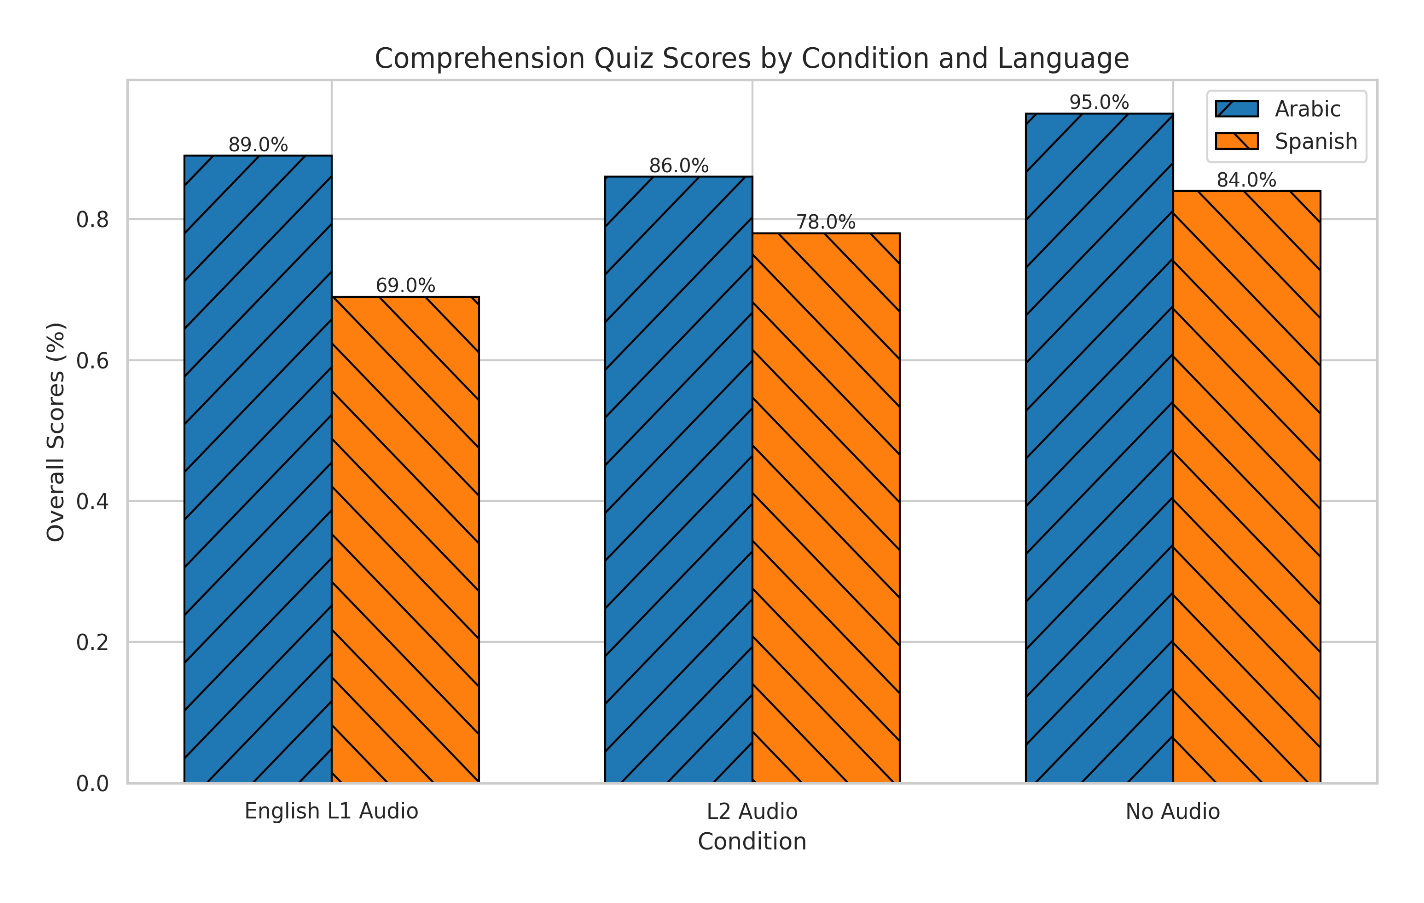
\includegraphics[width=\textwidth]{image3.jpg}
 \caption{Close up of the chat box}
 \label{fig4}
 \source{Authors}
\end{minipage}
\end{figure}

While digital tools and the use of different devices can aid the feedback process \cite{bakla2020extensive, elola2017writing}, one of our participants, Andrômeda, credited the way her peer used technology during one of their interactions to have raised negative emotions, impacting the way she processed that feedback. Andrômeda and Vítor had already had a peer conference to discuss their written peer feedback for a summary; for their second session, discussing the peer feedback given for a review, Vítor decided to use a second computer, where he had the text they were discussing opened. Vítor had a computer screen in front of him, where he saw and talked with Andrômeda, and another computer screen on his right-hand side, where he had the text in discussion. Andrômeda said this situation was uncomfortable as she always looked at her computer screen while speaking to Vítor. However, there were times in which Vítor, though interacting with her, was looking to the side at a different screen (\Cref{fig5}). During these moments, Andrômeda reported she did not know how to behave since it was strange to look at her interlocutor while he was not paying attention to her, or at least not making any eye contact. As a result, this second conference had more pauses while this pair was discussing.

\begin{figure}[h!]
\centering
\begin{minipage}{.8\textwidth}
 \includegraphics[width=\textwidth]{Fig4.jpeg}
 \caption{Screenshot of Vítor looking at a second screen}
 \label{fig5}
 \source{Authors}
\end{minipage}
\end{figure}

In addition to that, Andrômeda mentioned another shortcoming of the online conference. There were a few occasions in which they disagreed on some issues and left them to be resolved after the session. Likewise, Jay, who also did not share the screen when working with Mary Jay and kept only the verbal exchange, reported a few outstanding points after the peer conference. Notably, some of these issues were form-related and could have been solved by checking on a different source during their conferences (see next paragraph), which was the approach Ruth and Carina had to the task. The latter mainly solved their linguistic doubts during the conference.

Concerning the unresolved linguistic issues mentioned above, there was a lack of trust in the feedback giver, a learner of EAL. There were some instances in which the participants justified their comments by mentioning implicit knowledge about a given structure or word choice. Sentences such as “I don’t know exactly why you cannot use ‘although’ there, but I know you can’t.” (Andrômeda) or “I made this comment only because I have a feeling that this is not a possible collocation in English.” (Mary Jay) were common during their talks. At times, the writer would agree and say something like “Yes! You’re right! My mistake”, but there were times in which they would discuss the suggestion, and the writer would question the assertiveness of the reviewer as the feedback was solely based on a ‘hunch’. Probably a large percentage of these doubts could have been cleared by opening a new tab and consulting an English grammar website or an online dictionary. Nonetheless, these students did not resort to these affordances.


\subsection{WhatsApp as a bridging tool}

Although this study focused primarily on synchronous peer feedback conferences, during the individual interviews conducted with the participants, WhatsApp stood out as a key tool for feedback among these learners. In the following passage, Vítor illustrates the use of WhatsApp:

\begin{quote}
    We have our WhatsApp group. When we’re writing an essay and we’re not sure (about something), we write a comment there: “I think this would be good but I’m not sure” and if the person doesn’t understand it, then, we record an audio message on WhatsApp and then we research and send some prints of some sentences that use the structure […]
\end{quote}

In this excerpt, the use of WhatsApp indicates a smooth transition not only between devices (computer to mobile) but also in mode (written and aural). In addition, different linguistic resources from different sources seemed to be pooled according to a given student’s needs in a dynamic way to achieve their goals, which is in line with the idea of multiliteracies and several digital pedagogical openings \textcite{cope2013towards} highlight, e.g., ubiquitous learning and collaborative intelligence. The choice of using WhatsApp reinforces \textcite{chandra2021online} argument that traditional internet tools are not as timely and effective in terms of resources to solve problems students currently have.

Likewise, in a different use of WhatsApp – this time between a specific writer and reviewer – Ruth reported that she decided to send an audio message to her peer in response to the written feedback she received. She highlighted that the process of “externalising her idea” (i.e., transforming thought into language) was critical for her understanding of how she could have written a passage in her text. After the conversation with her peer, Ruth accessed this audio one more time, and, in her words, it was an enlightening experience:

\begin{quote}
    [...] because I externalised what I meant and then, from this audio, I understood how I should have written that passage. It was really cool. After I externalised that orally, trying to explain to the person (what I meant), I could rewrite this part of the text in a more understandable way.
\end{quote}

WhatsApp was as integrated into the (re)writing process as it was into their academic and social lives. According to Vítor, their WhatsApp group – with classroom friends – works as a forum where feedback is requested for a wide range of purposes, from university assignments to personal problems. In \textcite{bankier2022socialization}, learners preferred face-to-face meetings to discuss their academic writing practices outside class. In the present study, in which the pandemic restricted interactions, our participants supported WhatsApp as a tool for seeking feedback, like the findings in \textcite{umamah2022efl}.

Still, another role played by WhatsApp in the feedback process was to alleviate likely negative emotions aroused by the initial perception when looking at the written feedback received from a peer. Three of the six participants used the instant message tool for this purpose. They either sent individual audio messages with their written feedback to warn their pair that, although there were many comments in the document, it did not mean their text was of lower quality or sent messages in classmate-WhatsApp groups praising their peer’s text. Both actions were appreciated by the writers as, according to them, they lowered anxiety levels.

\section{Discussion}

This study probed students' use of digital affordances during online peer conferences to discuss written feedback implemented in an Academic Literacies course in English at a Brazilian university. We started investigating their previous experience with EAL writing, which indicated, similarly to \textcite{umamah2022efl}, an array of digital tools used during the writing process. Some of these tools were those used to scaffold one's writing (e.g., Grammarly and Thesaurus), while others were used by the learners to share their textual production asking others for feedback (Google Drive/Docs and WhatsApp). A trigger for using such tools was the fear of not writing up to expected academic standards. Thus, double-checking, using automated or peer feedback, was not a novelty for these students before the course.

Nevertheless, the findings suggest that online peer conferences to discuss peer feedback fell short of harnessing online affordances that could have helped some students. While one pair took advantage of digital openings by sharing their screen, so they could 'fix' and modify their texts while discussing automated feedback by Grammarly as well as using the chat box on Google Meet, i.e., simultaneously using different semiotic resources \cite{belda2021enhancing} to resolve issues collaboratively \cite{cheung2022verbal, cope2017learning}, the other two pairs had the text on their own screen while discussing them, and left many decisions to be made after the conference. One could argue that the pair who shared their screen and modified the text as they were discussing was strategic in terms of saving time once they had their final version of the text ready by the end of the peer conference; on the other hand, it might be that the other pairs did not take advantage of this affordance for specific reasons. One of the possible reasons for not sharing their screen, to show the text they were discussing, may have been a strategy used by participants to save face \cite{goffman1967interaction}, thus avoiding negative emotions. One participant – Andrômeda – declared that while the conference with the pair was positive because it allowed them to present arguments for their feedback regarding areas of disagreement, it was better to make final decisions individually afterwards.

In addition, the findings enrich the current field of peer feedback on EAL writing and the use of technology for learning to write by highlighting the pivotal bridging role WhatsApp had for academic purposes. From a multiliteracies paradigm, language and other forms of meaning are dynamic and constantly shaped by users to achieve their goals \cite{newlondon1996}, for example, recording a message – rather than sending a text – on WhatsApp. While face-to-face meetings to discuss academic practices are preferred \cite{bankier2022socialization}, critical moments led to adaptive actions such as switching to WhatsApp. In this respect, WhatsApp offered a multimodal channel where audio messages, links, and screenshots were shared between peers or in groups. If, in \textcite{bakla2020extensive}, learners reported difficulties comprehending audio feedback as they lacked visual support and preferred the computer rather than mobile devices, in the present study, audio messages seemed to work in tandem with written feedback. It was not a question of choosing the best device; different feedback modes and media served different purposes and offered more opportunities to develop feedback literacy \cite{carless2018development}.

In this respect, feedback through WhatsApp was not simply a supporting tool, it was a multimodal space created by learners to seek informal peer feedback \cite{yang2021feedback}. As mentioned by Ruth, it also worked as a tool for self-regulation when she revised her text using the audio message she had previously recorded to her pair. In other words, these messages may also serve as a spring for learning. The process of voicing her explanation not only solved communication issues between Ruth and Carina but was later retrieved by Ruth, showing the dynamic nature of output becoming input \cite{newlondon1996}. In addition, audio messages were also sent in advance as a buffer against possible negative emotions caused by one's written feedback.

The findings point to a few drawbacks concerning technology usage. By using two laptops, Vítor left Andrômeda feeling embarrassed, and, as a result, there were more pauses and moments of silence. \textcite{belda2021enhancing} argues that avoiding such moments in online interaction is crucial as they might affect communication flow. Moreover, the fact two pairs did not make the best use of digital affordances during their conference is also a drawback, considering that some issues they had were form-related and might have been solved by looking at different online sources during the conference. As there was no information or link to corroborate form-related feedback, a few students, such as Jay, reported a lack of confidence in this type of feedback. This fact is particularly negative, as \textcite{hattie2007power} argue that corrective surface-level feedback without confirmatory information does not allow such feedback to be incorporated and used in future tasks.

In terms of the pedagogical openings of digital learning pointed out by \textcite{cope2013towards, cope2017learning} – ubiquitous learning; active knowledge making; multimodal meaning; collaborative intelligence; metacognition; differentiated learning; and recursive feedback – it was possible to observe the presence of all of them in the interactions between the pairs, even though, as mentioned above, there was one pair of learners that seem to have made the most of this experience, and all affordances can be identified in their interaction. We can see, for example, ubiquitous learning happening when they make use of WhatsApp at different moments in the day to send each other's messages, knowledge being built actively when they use Grammarly, multimodality being used when a participant, besides seeing the image of her pair and talking to her, opted to use the chat box to send an excerpt of text, collaborative intelligence, which was constant throughout the whole activity, being used, for example, when one writer had a doubt and different colleagues went after the solution for that, metacognition explicitly being used when a writer highlighted the part of the text she wanted to revise later, differentiated learning when one pair decided to share their text on the screen and work on it while the conference was going on and the others kept their texts only in their individual screens, and recursive feedback (inherent to the task itself) intensively used when Sara used Grammarly when writing her text (automated feedback), then received written comments about the text from her pair (peer feedback), and finally reflected about a given portion of the text once again (self-feedback) before deciding on its final form.

\section{Conclusion}

Given the exploratory nature of this study, conducted in an online course due to the COVID pandemic, where the focus was to analyse rather than to direct tertiary learners to use specific digital tools, we draw two main conclusions from the findings. First, to harness the full potential of multimodal feedback in online peer conferences, generation Z learners might benefit from direct instruction and modelling on online tools and affordances \cite{cheung2022verbal, elola2017writing, yang2021feedback} that can ease and maximise peer feedback in such an online environment.

Second, informal forms of digital peer feedback using WhatsApp showed such feedback’s nuanced and complex role, which affected affective and cognitive aspects. WhatsApp, used in its multimodal pedagogical potential, bridged gaps these students found during the peer feedback process.

Pedagogical implications are two-fold; on the one hand, learners could benefit from explicit instruction on screen sharing the text and digital affordances during online peer conferences. On the other hand, course designers can enhance their practice by purposefully embedding informal peer feedback, especially through WhatsApp, into the writing process. However, caution is advised as learners in this study were acquainted with each other and, in some cases, were close friends. The use of WhatsApp for feedback, among some pairs, was common practice for almost every aspect of their lives, university assignments being part of this universe.

Finally, our data analysis shows the dynamic nature of communication, which requires teachers and learners to be open to embracing various forms of communication not limited to classroom physical space and time. However, agreement on what media to use and how to avoid communication overload is advised considering the situatedness \cite{santos2021kersch} aspect of academic literacies. Additionally, this discussion should inform learners of all assessment purposes this communication, even informal, will be used.

Due to its scope and methodology, this research did not compare groups of learners, e.g., instructed versus uninstructed use of digital affordances and learners who used WhatsApp versus those who did not. Future studies might consider a more controlled approach allowing for more robust claims on performance and learning.

\section{Funding}
This study was supported by CNPq.


\section{Acknowledgements}
We thank the participants of this study for their invaluable contribution, as well as the two anonymous reviewers and the Texto Livre editorial team.   

\printbibliography\label{sec-bib}
% if the text is not in Portuguese, it might be necessary to use the code below instead to print the correct ABNT abbreviations [s.n.], [s.l.]
%\begin{portuguese}
%\printbibliography[title={Bibliography}]
%\end{portuguese}


%full list: conceptualization,datacuration,formalanalysis,funding,investigation,methodology,projadm,resources,software,supervision,validation,visualization,writing,review
\begin{contributors}[sec-contributors]
\authorcontribution{Donesca Cristina Puntel Xhafaj}[supervision,formalanalysis,writing,review]
\authorcontribution{Rafael Zaccaron}[conceptualization,datacuration,formalanalysis,writing,review]
\end{contributors}



\end{document}

